% -----------------------------------------------------------------------------
%   Arquivo: ./02-elementos-textuais/resultadosEsperados.tex
% -----------------------------------------------------------------------------


\chapter{Avaliação da escalabilidade}
\label{chap:exp_preliminares}

Apresentadas as correções e aprimoramentos feitos na arquitetura D-Optimas, é necessário avaliar os impactos no seu funcionamento e comportamento. Neste capítulo será apresentada uma  bateria de experimentos, com o objetivo de avaliar a escalabilidade da nova implementação baseada em \textit{akka-cluster}.

A \autoref{sec:desempenho} descreve o experimento para avaliar o impacto do aumento da quantidade de nós do \textit{cluster} na execução da simulação, principalmente na latência entre as mensagens trocadas e a taxa de produção de soluções dos agentes. A \autoref{sec:resultado} apresenta os resultados obtidos e a análise estatística para cada tipo de mensagem analisada. Espera-se que, mantendo o número de agentes e o limite de regiões, mas aumentando o número de nós, a carga seja melhor distribuída entre os nós, e que o tempo médio entre um envio de uma mensagem por um ator e o seu respectivo processamento em outro ator diminua. Por fim, a \autoref{sec:sintese} apresenta uma síntese dos resultados. 

\section{Avaliação de desempenho da arquitetura}
\label{sec:desempenho}

Esse experimento avaliou a média da latência das trocas de mensagens entre os agentes, regiões e atores supervisores da simulação. O número de nós do \textit{cluster} em que a arquitetura executou foi o único parâmetro que sofreu variação. 

Foram executadas 4 instâncias, nomeadas S3, S4, S5 e S6, utilizando de 3 a 6 nós. Para cada instância do experimento foram obtidas 14 réplicas da mesma configuração, que é exibida no \autoref{tab:expS}. Cada execução contou com 18 agentes, sendo 6 agentes construtores, 6 populacionais e 6 agentes de busca local. Os agentes construtores tiveram o tempo de vida limitado à 200 unidades pois as soluções por eles geradas servem somente como soluções iniciais.
Para este experimento os mecanismos de aprendizagem e memória dos agentes foram desabilitados, uma vez que a mudança na organização do sistema impacta fortemente no funcionamento desses componentes. 
Além destas configurações, ficou estabelecido o número limite de 100 regiões no sistema, o número mínimo de 30 soluções para uma região se particionar, e o tempo limite de 1000 unidades para que a simulação fosse interrompida.

O ambiente computacional utilizado foi o \textit{cluster} do Laboratório de Sistemas Inteligentes (LSI) do CEFET, composto de seis máquinas com processador Intel i7, 32GB de RAM e 2TB de HD cada. O sistema operacional utilizado foi o CentOS 6, e o SLURM como escalonador
de tarefas. A versão do JDK (\textit{Java Development Kit}) utilizada foi a 12.0.1.

\begin{table}
\caption{\label{tab:expS}Parâmetros das meta-heurísticas}
\centering

\begin{tabular}{lllc}
    \toprule
    \textbf{Nº de agentes}  & \textbf{Metaheurística}   & \textbf{Parâmetro}        & \textbf{Valor} \\
    \midrule
    \multirow{2}{*}{6}      & \multirow{2}{*}{GRASP}    & iterações                 & 100\\
                            &                           & iterações busca local     & 100\\
                            &                           & alpha                     & 0.5\\
    \midrule
    \multirow{2}{*}{3}      & \multirow{2}{*}{ILS}      & iterações                 & 500\\
                            &                           & nível de distúrbio        & 10\\
    \midrule
    \multirow{2}{*}{3}      & \multirow{2}{*}{ILS}      & iterações                 & 500\\
                            &                           & nível de distúrbio        & 7\\
    \midrule
    \multirow{4}{*}{3}      & \multirow{4}{*}{GA}       & iterações                 & 300\\
                            &                           & tamanho da população      & 20\\
                            &                           & taxa de mutação           & 0.2\\
                            &                           & taxa de cruzamento        & 0.7\\
    \midrule
    \multirow{4}{*}{3}      & \multirow{4}{*}{GA}       & iterações                 & 500\\
                            &                           & tamanho da população      & 30\\
                            &                           & taxa de mutação           & 0.1\\
                            &                           & taxa de cruzamento        & 0.8\\
    \bottomrule
\end{tabular}
\end{table}

Foram escolhidos quatro tipos de mensagem para serem analisadas. A primeira escolhida foi \textbf{UpdateGlobalSummary} que é frequentemente enviada pelo líder da simulação a todas as regiões e agentes sempre que alguma mudança acontece no sistema. A segunda mensagem, do tipo \textbf{UpdateRegionSummary}, é enviada por uma região sempre que recebe uma nova solução, ou uma fissão ou fusão acontece. A terceira mensagem analisada, do tipo \textbf{RegionSplit}, é enviada pelas regiões ao líder da simulação sempre que uma região se particiona, e por fim, a quarta mensagem mensagem, do tipo \textbf{SolutionResponse}, é enviada aos agentes pelas regiões em resposta a uma solicitação de soluções. Neste subconjunto de mensagens  estão presentes as principais e mais frequentes interações entre os agentes, regiões e o líder. Os dados extraídos foram tratados, removendo eventuais anomalias (latências negativas, por exemplo) e a média das latências para cada execução, para cada tipo de mensagem, e foram computadas a média das latências para cada execução e para cada tipo de mensagem. 

Antes de apresentar e discutir os resultados, é necessário fazer uma observação acerca do tratamento dos dados. Entre as execuções, cada mensagem pode ter sido trocada um número diferente de vezes e algumas delas podem não ter sido recebidas. Isso faz com que a média das latências da mensagem do tipo \textbf{UpdateGlobalSummary} em uma execução tenha sido calculada com um número diferente de observações em cada uma das 14 repetições para cada um dos 4 fatores. Esse particularidade dos dados, somada à estocasticidade inerente à arquitetura, pode levar os dados a não se comportarem bem, ainda que essa amostragem esteja congruente com a definição do teorema do limite central. Dito isso, as premissas da ANOVA são verificadas para cada tipo de mensagem, e quando atendidas, o teste paramétrico é escolhido. Todos os testes estatísticos foram realizados com um nível de confiança de 95\%.


\section{Resultados do experimento}
\label{sec:resultado}

\begin{figure}
    \centering
    \caption{\textit{Boxplot} das médias das latências da mensagem \textbf{UpdateGlobalSummary} para 14 execuções da arquitetura D-Optimas com duração de 1000 unidades de tempo discreto em 3, 4, 5 e 6 nós do \textit{cluster} }
    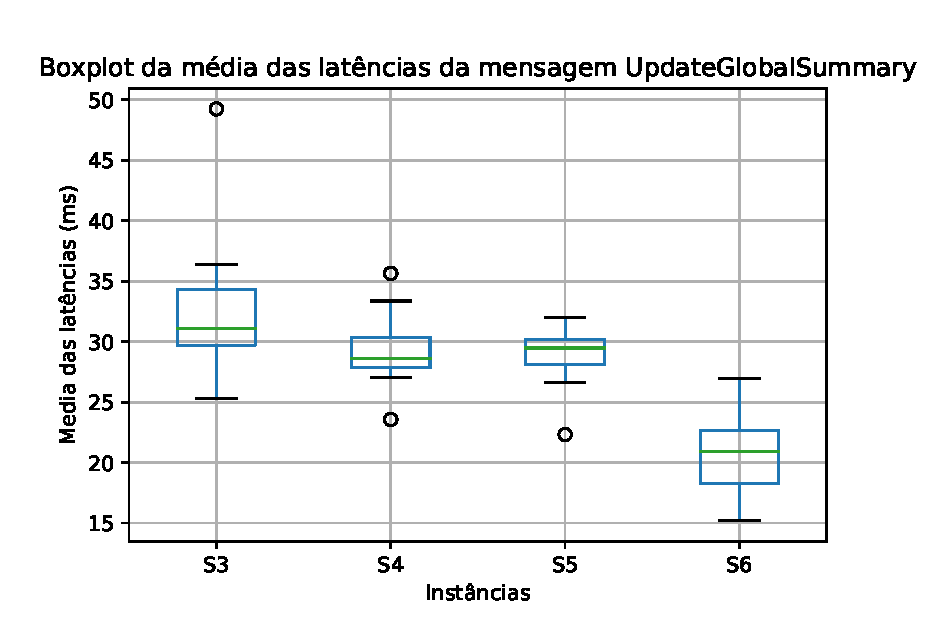
\includegraphics[scale=0.8]{imagens/update_global_summary.eps}
    \label{fig:update_global_summary}
\end{figure}

A \autoref{fig:update_global_summary} exibe o \textit{boxplot} das médias das latências das mensagens do tipo \textbf{UpdateGlobalSummary}. Visualmente é possível perceber que os dados estão bem comportados e há uma tendência de queda da latência a medida que o número de nós cresce. 

Para esse subconjunto dos dados, dois dos três pressupostos da ANOVA foram atendidos. O teste de Levene acusou um p-valor de $0.31538$, falhando em rejeitar a hipótese nula de que a variância dos resíduos é homogênea. Os resíduos são independentes mas não seguem uma distribuição normal, pelo teste de Shapiro-Wilk (p-valor de $0.000161$). Como a ANOVA é robusta a pequenas variações na normalidade, este teste foi escolhido. O p-valor obtido foi de $0$, indicando que há diferença em pelo menos uma das médias. 

A \autoref{tab:update_global_summary_tukey} exibe os resultados do teste de Tukey-HSD, para um nível de significância de $5\%$. O teste conclui que não há diferença entre as instâncias S3 e S4, e S4 e S5, onde há variação de apenas um nó no \textit{cluster}.

\begin{table}[ht!]
    \centering
    \caption{Comparações par-a-par (teste de Tukey-HSD) para as médias das latências de mensagens do tipo \textbf{UpdateGlobalSummary}}
    \begin{tabular}{cccc}
    \toprule
    \multicolumn{2}{c}{\textbf{Instâncias}} & \textbf{p-valor} & \textbf{Rejeita $H_0$?}\\
    \midrule
    S3   &  S4  & 0.0938 &  Não \\
    S3   &  S5  & 0.0451 &   Sim \\
    S3   &  S6  &  0.001 &   Sim \\
    S4   &  S5  &    0.9 &  Não \\
    S4   &  S6  &  0.001 &   Sim \\
    S5   &  S6  &  0.001 &   Sim \\
    \bottomrule
    \end{tabular}
    \label{tab:update_global_summary_tukey}
\end{table}

A segunda mensagem analisada foi a \textbf{UpdateRegionSummary}. A \autoref{fig:update_region_summary} exibe a distribuição das médias das latências para as quatro instâncias do experimento. Aparentemente há uma tendência de diminuição da variância a medida que a arquitetura escala. Os dados não atendem aos pressupostos de normalidade (com p-valor de $0.000121$) e homocedasticidade (p-valor de $0.004774$).  

Por isso, foi escolhido um teste não paramétrico de Kruskal-Wallis, para verificar se há diferença entre as instâncias. O teste produziu um p-valor de $0.002919$, que leva a rejeição da hipótese nula, indicando que há diferença em pelo menos uma das médias. 

\begin{figure}
    \centering    
    \caption{\textit{Boxplot} das médias das latências da mensagem \textbf{UpdateRegionSummary} para 14 execuções da arquitetura D-Optimas com duração de 1000 unidades de tempo discreto em 3, 4, 5 e 6 nós do \textit{cluster} }
    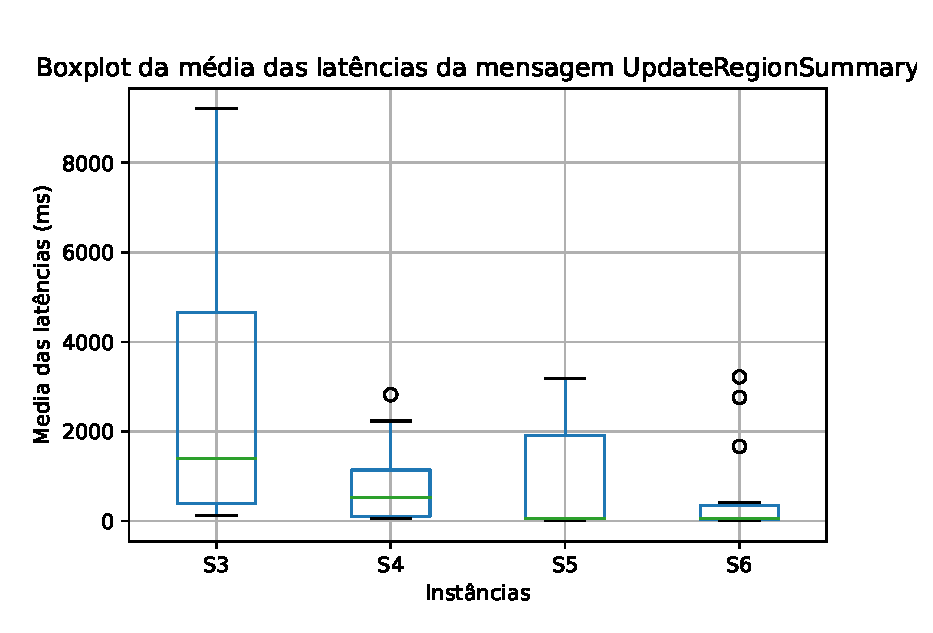
\includegraphics[scale=0.8]{imagens/update_region_summary.eps}
    \label{fig:update_region_summary}
\end{figure}

Para verificar em qual dos pares está a diferença, foi escolhido um teste \textit{post-hoc} não paramêtrico de Conover-Iman. Os p-valores obtidos pelo teste são apresentados na tabela \autoref{tab:update_region_summary}. É possível observar que há diferença sempre que se adiciona pelo menos dois nós na simulação.

\begin{table}[ht!]
    \centering
    \caption{Comparações par-a-par (Teste de Conover) para a média das latências de mensagens do tipo \textbf{UpdateRegionSummary}}
    \begin{tabular}{cccc}
    \toprule
    \multicolumn{2}{c}{\textbf{Instâncias}} & \textbf{p-valor} & \textbf{Rejeita $H_0$?}\\
    \midrule
     S3 &    S4 &  0.06021 &  Não  \\
     S3 &    S5 &  0.00378 &   Sim \\
     S3 &    S6 &  0.00017 &   Sim \\
     S4 &    S5 &  0.27176 &  Não  \\
     S4 &    S6 &  0.03905 &   Sim \\
     S5 &    S6 &  0.31895 &  Não  \\
     \bottomrule
    \end{tabular}
    \label{tab:update_region_summary}
\end{table}

A terceira mensagem  analisada foi a \textbf{RegionSplit}. O \textit{boxplot} das médias das latências para as quatro instâncias do experimento é apresentado na \autoref{fig:region_split}. Novamente é possível observar uma tendência de queda da latência a medida que novos nós são adicionados à simulação. Os pressupostos de normalidade e homocedasticidade não são atendidos, com p-valores de $0.000005$ e $0.002790$, respectivamente.  

\begin{figure}
    \centering
    \caption{\textit{Boxplot} das médias das latências da mensagem \textbf{RegionSplit} para 14 execuções da arquitetura D-Optimas com duração de 1000 unidades de tempo discreto em 3, 4, 5 e 6 nós do \textit{cluster} }
    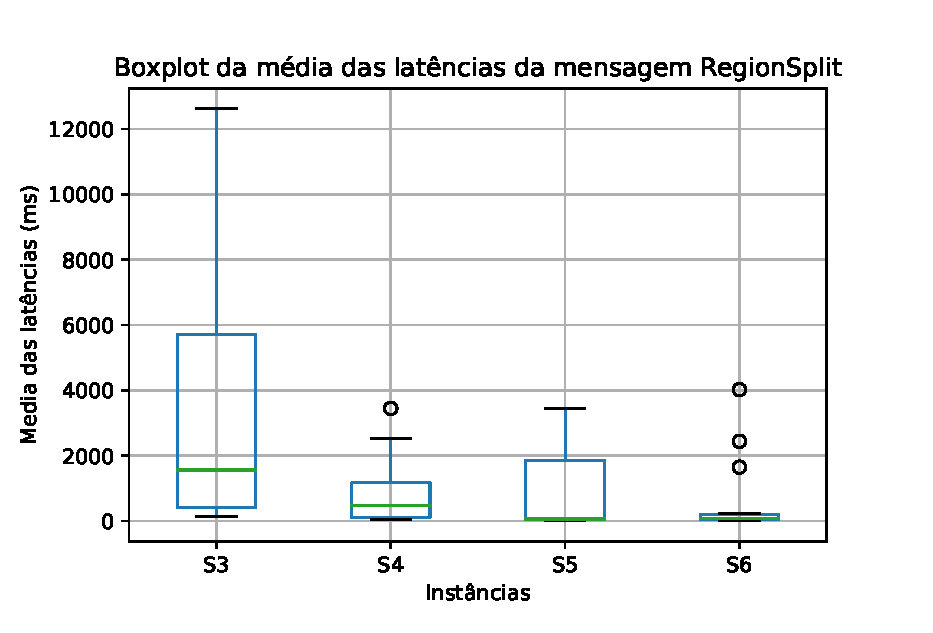
\includegraphics[scale=0.8]{imagens/region_split.eps}    \label{fig:region_split}
\end{figure}

O teste de Kruskal-Wallis produziu um p-valor de $0.0.002748$, o que indica uma diferença em pelo menos uma das médias. A \autoref{tab:region_split} apresenta os resultados do teste de Conover-Iman. O teste novamente indica que não é possível observar diferença na latência entre duas amostras com a variação de apenas um nó. Adicionando 2 nós, a diferença entre as médias da latência é significativa. 

\begin{table}[ht!]
    \centering
    \caption{Comparações par-a-par (Teste de Conover) para a média das latências de mensagens do tipo \textbf{RegionSplit}}
    \begin{tabular}{cccc}
    \toprule
    \multicolumn{2}{c}{\textbf{Instâncias}} & \textbf{p-valor} & \textbf{Rejeita $H_0$?}\\
    \midrule
       S3  &  S4  &  0.06021  &  Não \\
       S3  &  S5  &  0.00378  &   Sim \\
       S3  &  S6  &  0.00017  &   Sim \\
       S4  &  S5  &  0.27176  &  Não \\
       S4  &  S6  &  0.03905  &   Sim \\
       S5  &  S6  &  0.31895  &  Não \\
     \bottomrule
    \end{tabular}
    \label{tab:region_split}
\end{table}


Finalmente, a distribuição das médias das latências para as mensagens do tipo \textbf{SolutionResponse} são exibidas na \autoref{fig:solution_response}. Pela análise gráfica é possível dizer que há diferença entre a instância S3 e S4, S5 e S6. As observações são independentes e as variâncias são homogêneas (com p-valor de $0.060870$). 

\begin{figure}
    \centering    
    \caption{\textit{Boxplot} das médias das latências da mensagem \textbf{SolutionResponse} para 14 execuções da arquitetura D-Optimas com duração de 1000 unidades de tempo discreto em 3, 4, 5 e 6 nós do \textit{cluster} }
    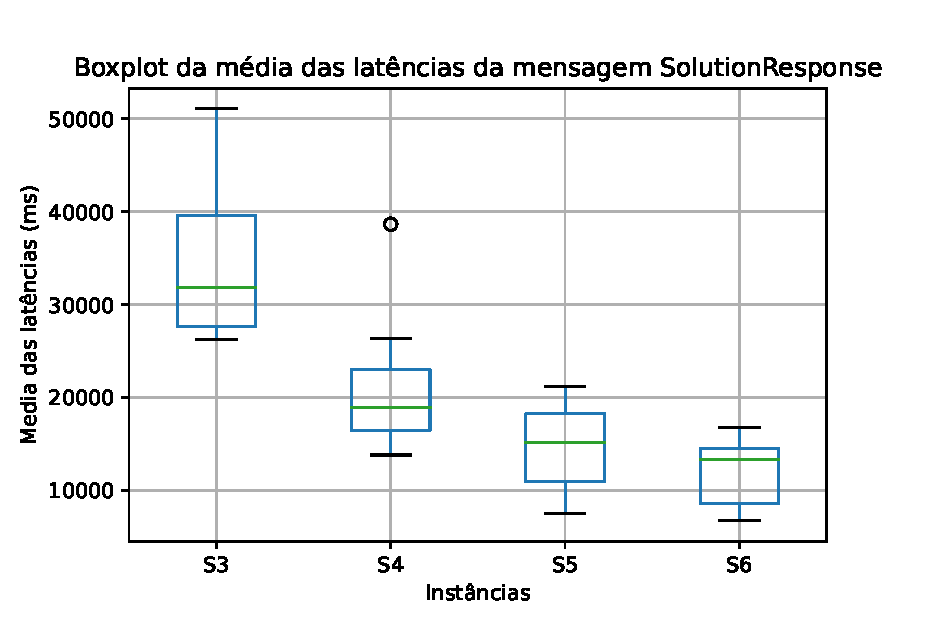
\includegraphics[scale=0.8]{imagens/solution_response.eps}
    \label{fig:solution_response}
\end{figure}

Há um pequeno desvio na normalidade, o que permite executar uma análise paramétrica. A ANOVA indica que há diferença entre as médias, com p-valor igual a $0$. A \autoref{tab:solution_response} indica que há diferença entre S4 e S6, além da diferença entre S3 que já era percebida na análise gráfica. 

\begin{table}[ht!]
    \centering
    \caption{Comparações par-a-par (Teste de Tukey-HSD) para a média das latências de mensagens do tipo \textbf{SolutionResponse}}
    \begin{tabular}{cccc}
    \toprule
    \multicolumn{2}{c}{\textbf{Instâncias}} & \textbf{p-valor} & \textbf{Rejeita $H_0$?}\\
    \midrule
    S3  &  S4 & 0.001   & Sim  \\
    S3  &  S5 & 0.001   & Sim  \\
    S3  &  S6 & 0.001   & Sim  \\
    S4  &  S5 &  0.0862 & Não \\
    S4  &  S6 &   0.004 & Sim  \\
    S5  &  S6 &  0.6325 & Não \\
     \bottomrule
    \end{tabular}
    \label{tab:solution_response}
\end{table}

\section{Síntese do resultado}
\label{sec:sintese}

% aumentar o tamanho do cluster sem aumentar a simulação fornece mais recursos, favorece o balanceamento de carga, e leva os atores a processarem mais rápido
De uma maneira geral, aumentar o tamanho do \textit{cluster}, mantendo a quantidade de agentes e o limite de regiões, significa oferecer mais recursos computacionais à arquitetura. A presença de mais núcleos de processamento, memória, largura de banda, favorece o balanceamento de carga. Ao distribuir melhor a carga entre os nós de processamento, é natural que o  escalonamento entre os atores, o tempo de espera por I/O e a paginação de memória diminuam, fazendo que cada execução do ator seja mais eficiente.

% os resultados mostram que há de fato uma tendência de queda quando o número de nós aumenta, e o número de entidades é mantido o mesmo
Dito isto, os resultados mostram que há de fato uma tendência de queda da latência média com o aumento do número de nós, em especial, sempre que mais de um nó é adicionado na simulação. Em outras palavras, os atores são mais rápidos em processar as mensagens que recebem. Essa tendência é um indício de que a arquitetura foi construída de maneira a aproveitar de maneira eficiente os recursos que estão disponíveis para ela. 

% mensagens que são recebidas pelo líder tem variância menos homogêneas, mas ainda assim parece haver uma tendência de queda a medida que o líder tem mais recursos computacionais
Entre os quatro tipos de mensagem analisadas neste experimento é possível observar que há uma diferença na ordem de grandeza e na variância comparando as mensagens recebidas pelo líder e as recebidas por outras entidades da simulação. É possível que este fenômeno seja reflexo de uma concentração de tarefas no líder. Mesmo que as tarefas não tenham uma complexidade computacional alta (a maioria delas possui complexidade assintótica da ordem $\mathcal{O}(n)$, onde $n$ é o número de agentes e regiões na simulação), pode haver uma demora em atender as mensagens que se acumulam rapidamente. Ainda assim, é possível observar que o líder se beneficia também do aumento de recursos computacionais, diminuindo a média da latência.

% para de fato verificar o potencial de escalabilidade da arquitetura, é necessário executar outros testes, variando outros fatores, por exemplo, o número máximo de regiões e o número de agentes em execução.
É preciso ressaltar que os resultados obtidos neste experimento não indicam uma escalabilidade da arquitetura sob qualquer condição. Os resultados são preliminares e dão bons indícios da resiliência da arquitetura como um sistema distribuído, mas para obter resultados mais robustos é necessário avaliar outros fatores, como por exemplo, o número máximo de regiões permitidas, o número de agentes em execução e o crescimento do conjunto de soluções produzido pela arquitetura. Além disso, é necessário avaliar o funcionamento da arquitetura num \textit{cluster} com dezenas ou centenas de nós. 

% esta avaliação é importante para verificar a eficiência do software, principalmente para oferecer a solução a um usuário final. De toda forma, este é um sistema de tempo discreto, uma latência baixa é desejável, mas não influência na qualidade das soluções. 
Avaliar o desempenho da D-Optimas é importante para certificar a correta implementação como um sistema distribuído, bem como a eficiência do \textit{software}, principalmente para oferecê-lo como uma ferramenta de trabalho para um usuário final, um tomador de decisão num processo de otimização. De todo modo, este é um sistema de tempo discreto, todas as meta-heurísticas são algoritmos discretos, que não dependem de resposta em tempo real. É claro que uma latência baixa é desejável, mas ela de fato não influencia na qualidade das soluções, somente no tempo de espera por soluções de boa qualidade.


\begin{comment}
\section{Avaliação do efeito da memória na qualidade das soluções produzidas}
% - O que esse experimento avaliou 
Este segundo experimento avaliou o efeito da adição da memória \textit{Q-learning} na qualidade das soluções produzidas pela arquitetura D-Optimas. 
% - Quais amostras foram coletadas
Para tanto, foram executadas duas configurações da arquitetura. A primeira configuração com a memória desabilitada, doravante denominada \textbf{NQ}, que servirá como \textit{baseline}. O segundo nível do experimento, de sigla \textb{Q}, corresponde à memória Q-learning habilitada em todos os agentes populacionais e buscas locais, com uma taxa de utilização da memória de 80\%.

% - Qual foi a configuração deste experimento
Para cada nível do experimento foram coletadas 19 amostras do melhor valor da função objetivo ao longo do tempo. Cada execução contou com 18 agentes, sendo 6 agentes construtores, 6 populacionais e 6 agentes de busca local. Os agentes construtores tiveram o tempo de vida limitado à 200 unidades pois as soluções por eles geradas servem somente como soluções iniciais. Os parâmetros de configuração de cada agente estão descritos na \autoref{tab:expQConfig}.
% - Quais os dados foram colhidos das amostras
Foram coletados os 19 melhores valores da função objetivo encontrados ao final de cada execução.  
% - Quais as ressalvas eu devo fazer a esse experimento

\begin{table}[]
    \centering
    \begin{tabular}{ccc}
         \textbf{Metaheurística}&\textbf{Parâmetro} & \textbf{Valor}  \\
         \multirow{3}{*}{GRASP}     & iterações             & 500   \\
                                    & iterações busca local & 100   \\
                                    & alpha                 & 0.5   \\
         \midrule
         \multirow{2}{*}{ILS}       & iterações             & 500   \\
                                    & distúrbio             & 7     \\
         \midrule
         \multirow{4}{*}{GA}        & iterações             & 500   \\
                                    & tamanho da população  & 30    \\
                                    & taxa mutação          & 0.2   \\
                                    & taxa de cruzamento    & 0.5   \\
         
    \end{tabular}
    \caption{Configuração dos agentes para o experimento que avaliou o efeito da memória \textit{Q-learning}}
    \label{tab:expQConfig}
\end{table}

\subsection{Resultado do experimento}


\subsection{Síntese do resultado}

\section{Considerações finais}

\end{comment}
